\chapter{About expression, visualisation, correlation and clustering}\label{ch:expression}
%\chapter{More quality checks and data preparation}

\begin{comment}
\setlength{\epigraphwidth}{\textwidth}%0.6
\setlength{\epigraphrule}{0pt}%0.1
\epigraphhead[70]{%
\epigraph{[..] 80\% of the data analysis task is spent on cleaning and
understanding the data.}{\cite{Dasu2003-bg}}%
}
\end{comment}

As a first step towards the different meta-analyses presented in this thesis,
I have opted for a semi-empirical approach to determine
a consensus set of methods and parameters on each individual study
before applying them across all the datasets in the further chapters.
This strategy has also allowed me
to estimate the overall data quality per dataset
and to structure them appropriately for the upcoming analyses.

I mentioned in \Cref{ch:datasets} quality checks
that happened before the processing of the data.
Those quality assessments are rather technical\footnote{Is it true signal
or noise?
Are all the nucleotides called?
Is it a true identification or a false positive?~\ldots}.
In the present chapter, I describe post-processing quality (or sanity) checks
that examine higher (and fuzzier) aspects, \eg:
%\KOMAoptions{parskip=never}
\begin{itemize}[topsep=0pt,nosep]
    \item Possible outliers in the data
    \item Systematic and unsystematic \emph{batch effect} within each study
    \item Adequacy of data, concepts and statistical models
\end{itemize}
%\KOMAoptions{parskip=half*}
Even if every of these aspects may not be addressed or corrected,
the final results and interpretations of this study are then more solid.

\section{Visualisation of expression data}

Data visualisation is a simple, but very effective method
towards adequate analyses and thus more pertinent results.
It allows uncovering the detection of underlying structures
and possible unwanted artefacts.

\subsection{Distribution plots}\label{subsec:distribPlot}
\vspace{-0.2in}
In the literature, expression values are frequently
visualised on a log-scale ($\log_{2}(x)$).
\Cref{fig:distribPlot}a and b illustrate how
this scaling improves the readability of the plot.
Furthermore, the log-scale allows one to transform count data to continuous
while smoothing the global distribution shape towards a normal distribution.
Thus, this transformation enables
the use of many readily available statistical models
that require normally distributed data.
Besides, others (\eg\ \citet{Danielsson2015-cn}) advocate
for logarithmic transformation before analysing interstudy samples.
To overcome the lack of definition of $\log_{2}(0)$,
I have added a common \emph{pseudocount} (equal to $1$)
to all the observations.
However, in a few cases and only for visualisation purposes,
I have removed the null values to avoid misinterpretations;
for examples the expression distribution (per tissue) plots
\Cref{fig:distribPlot,fig:distribTrans,fig:distribProt}.
When I remove the null values I clearly state it in the plot legend
as the norm is the pseudocount addition.

\begin{figure}[!htbp]
    \centering
    \includegraphics[scale=0.7]{expressed/IBMexpression.png}
    \caption{Untransformed and Log$_{2}$-transformed (null values removed) profile
    of expression levels (\FPKM, \pcgs\ only and all null values excluded)
    for the \ibm\ dataset}\label{fig:distribPlot}
\end{figure}

\begin{figure}[!htbp]
    \centering
    \includegraphics[scale=0.7]{expressed/transLog2_1.pdf}
    \caption{Profile of expression levels across the transcriptomic (\pcgs\ only)
    studies (null values removed)
    }\label{fig:distribTrans}
\end{figure}

\Cref{fig:distribTrans} shows all the remaining transcriptome datasets.
Overall,
on this $\log_{2}(x)$ scale (and with all null values excluded):
all the samples present a similar shape;
a peak near $0$ for the lowly expressed and undetected genes and a long-trailing tail.
The bulk of the expressed genes on this scale is below $6$ (\ie\ below 63 \FPKM).
In \Cref{fig:distribTrans}c, we can observe that the general expression
of the pancreas is shifted towards the left in comparison to the other tissues.
This may be an artefact as this shift of the values distribution
is absent in the pancreas of the other transcriptomic studies
(\Cref{fig:distribPlot}b and \Cref{fig:distribTrans}d).
Moreover, as highlighted by the next chapter analyses,
\uhlen's and  \gtex's pancreas are strongly
correlated ($r = 0.83$;$\rho = 0.96$).

\begin{figure}[!htbp]
    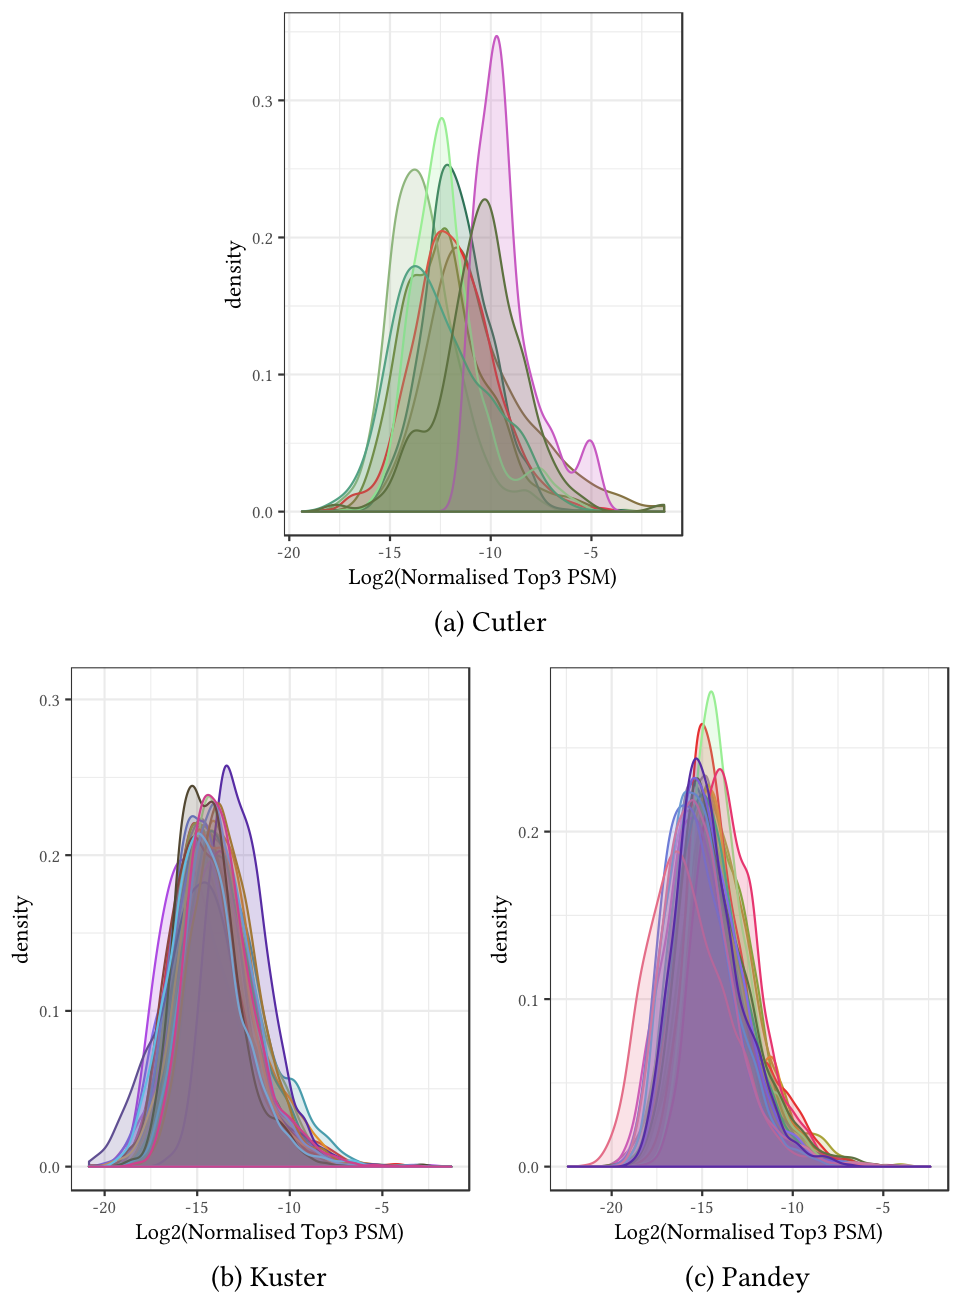
\includegraphics[scale=0.85]{expressed/protLog2.png}
    \caption{Profile of expression levels across the proteomic studies
    (null values removed)
    }\label{fig:distribProt}
\end{figure}

Aside from the \pandey\ data (\Cref{fig:distribProt}c),
the expression of the proteins is more heterogeneous
(in particular \cutler\ data, see \Cref{fig:distribProt}a).
This is concordant to the more disparate and variable techniques involved in
the proteomic sample preparation (see \Cref{subsec:ProtSampPrep}:
\nameref{subsec:ProtSampPrep}).

\subsection{Scatter plots}
\vspace{-0.1in}
\citet{anscombe} created four datasets (see \Cref{fig:Anscombe})
which share similar descriptive statistics to show the importance
of data visualisation even through a simple scatter plot.
He demonstrated that checking the datasets graphically with scatter plots
allows one to quickly detect outliers and roughly estimate
the relationship between two variables.
Even a non-linear but strong relationship is promptly highlighted
(\eg\ top right corner of~\Cref{fig:Anscombe}).

\begin{figure}[!htbp]
    \hspace*{-2cm}
    \begin{subfigure}[b]{0.61\textwidth}
      \centering  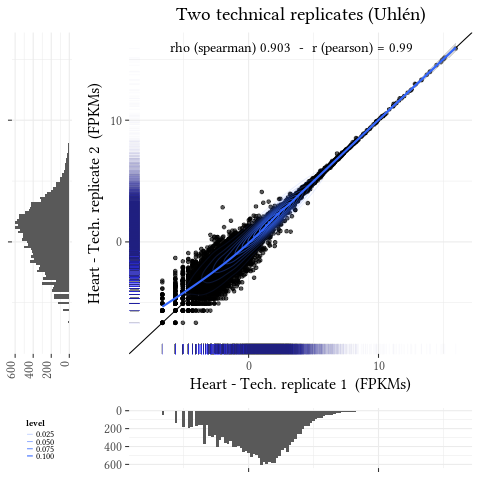
\includegraphics[width=\textwidth]{expressed/RepTechscat_heart.png}
        \caption{Technical replicates (Heart)}\label{fig:scatTechRep}
    \end{subfigure}~%
    \begin{subfigure}[b]{0.61\textwidth}
    \centering 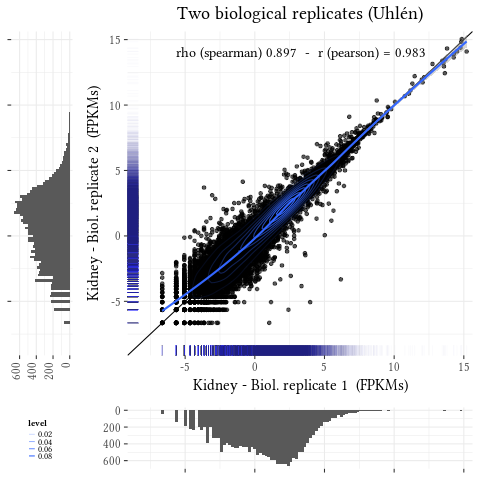
\includegraphics[width=\textwidth]{expressed/RepBiolscat_kidney.png}
        \caption{Biological replicates (Kidney)}\label{fig:scatBiolRep}
    \end{subfigure}
    \caption[Examples of scatter plot for replicates from \uhlen\ (transcriptome)
    ]{\textbf{Examples of scatter plot for replicates from \uhlen\ (transcriptome)}
     Technical replicates present very strong correlations particularly for
    higher expressed \mRNAs\ (≥ 32 \FPKM).
    Biological replicates present lower but still strong correlations within
    the same dataset.
    }\label{fig:scatEg}
\end{figure}

\Cref{fig:scatTechRep} illustrates how very lowly detected \glspl{RNA}
diverge even in technical replicates.
Biological replicates, within a same dataset,
may present very close profiles
even if the spread for the lowly genes
is even greater
as showed in \Cref{fig:scatBiolRep}.


\section{Main statistical approaches}

As the general normal distribution shape of the gene expression levels
on log-scale are similar,
I have also computed Pearson correlation coefficients
(in addition to Spearman ones)
to assess the similarity of the replicates
within (intra) and between (inter) studies.

\subsection{Correlation}
%Cum hoc ergo propter hoc

Correlation coefficients are a measure of the statistic dependence between two
continuous variables\footnote{In the context of this study, the variables are
either expression levels of a given gene across samples/tissues
or expression levels of all genes
\emph{between} two samples or tissues} (\eg\
$X$ and $Y$) and always ranges within $[-1,1]$ (see also
\cref{sec:CorrMore}: \nameref{sec:CorrMore}).

The correlation coefficient is computed by the pairwise comparison of observations
between two variables. Most implementation methods
will manage an unbalanced number of observations by excluding the incomplete pairs.
To ease the interpretation I filtered the data \latin{a priori};
I only kept expression values \emph{effectively observed}
in all the datasets
(as I explain in~\cref{sec:ExpressedOrNot}: \nameref{sec:ExpressedOrNot}).

From the several methods available to compute the correlation coefficient,
I chose both the Spearman and the Pearson correlations.
As Spearman correlations are computed on ranks,
they report any kind of relationship,
while Pearson correlations are computed on the values
and report only linear relationships.
However, Pearson correlations are easier to interpret
and can be used with one of the variable to predict the other one.
(See also \Cref{subsec:SpearmanCor}: \nameref{subsec:SpearmanCor} and
\Cref{subsec:PearsonCor}: \nameref{subsec:PearsonCor}).

\begin{figure}[!htpb]
    \includegraphics[scale=0.9]{expressed/repCorr}\centering
    \caption[Correlation coefficients between RNA-Seq replicates]{%
    \label{fig:repCorr}\textbf{Correlation coefficients between \Rnaseq\
    replicates.}
    The correlation means and medians are high across the studies replicates.
    However, the range of the correlations are quite extreme in a few
    case. Spearman correlations are higher than the Pearson ones.
    See also \Cref{subsec:PearsonVsSpearman}.}
\end{figure}

\Cref{fig:repCorr} (and \Cref{tab:repCorr}) presents
the Pearson and Spearman correlation coefficients
for the technical replicates for \uhlen\ study and
the biological replicates within \vt, \gtex\ and \uhlen\ studies.
On average the correlation coefficients are high both for the technical or
the biological replicates.
The \gtex\ study presents the same average correlation coefficients
but a more extreme range.
This may be explained by a strong batch effect as the samples were collected
and sequenced at different times by different laboratories.

\subsection{Clustering analysis}

As we know the tissue type for each sample of each dataset,
we may debate that supervised analyses can be more informative
than unsupervised ones.
However, they would involve proper corrections for batch effects and
other technical biases for each dataset.
This is challenging as it often requires more knowledge than what is available
through the repositories.
In \Cref{ch:datasets}, we have seen that is also unwise to rely solely on the
normalised data provided by the original authors
when working with various datasets
that are non-uniformly processed\footnote{Eventual bias
corrections in \Rnaseq\ vary according to planed downstream analyses and
proteomic data is hard to handle and two processing pipelines may rather give
quite different results (see~\Cref{subsec:IntegrationNewMethQuant}).}.

To assess the consistency of the quantification across the different datasets,
in particular for \Rnaseq,
I picked a widely used unsupervised method
for exploratory analysis in gene expression studies:
clustering analysis.
There are many available approaches and algorithms from which to pick;
I~chose a (bottom-up) \emph{hierarchical} clustering (a.k.a.\
\emph{connectivity-based} clustering).
This sort of clustering is widely used in gene expression studies.
%as it is relevant: embryologically (\eg\ for a multi-tissues study) within one organism
%or evolutionary when different species are compared.
Broadly speaking,
this method groups samples by similarity in an extensive hierarchy,
which allows uncovering possible hidden structures within the data;
thus establishing if samples are more alike biologically or by study origin
for instance.

In general, we expect biology to be a better predictor when we only consider
data from either transcriptome or proteome. Even more so if the
identification technology and the quantification workflows are
consistent. Yet, a technical predictor can not be directly excluded.
Indeed, most transcripts (in particular \mRNAs) are expressed in many tissues.
Two tissues chosen at random share about 60 to 90\% of their pool of
\mRNAs~\mycite{ramskoldan:2009,UhlenGastro}.
Parallelly, on the proteome side, \citet{PandeyData}
estimate that 75\% of the mass of a cell is due to ubiquitous proteins and
\citet{KusterData} estimate that about 10,000
to 12,000 proteins are ubiquitously detected, which represent about 60 to 75\%
of the proteins that they identified per tissue. Thus, if the variation of
expression are too subtle from one tissue to another, a strong sample collection
or data processing bias may hide any relevant biological signal.

In practice, each sample starts in its own cluster and then
iteratively, each cluster is merged with its nearest one.
The method has two parameters: the distance and the linkage method.
Debate is still going on how to pick these parameters among the many possible
choices (for more details see~\mycite{Jaskowiak2014,Guinand2002-ad}).

The distance measures the dissimilarity between two samples and one common
approach is to calculate the subtraction result of
the correlation coefficient from $1$ (hence, a greater similarity between the two
samples means a smaller distance).
In analogy to previous analyses, I have also used both Spearman
and Pearson correlation methods.

The linkage parameter specifies which part of each cluster is used as reference
for computing the distance between the clusters. There are many methods and after
trying several, I have arbitrary selected the one that divides most accurately
the samples by their tissue source across the different datasets.
In fact, I noticed that Ward's method~\mycite{Ward1963}
was the best for this task and was outperforming the complete-linkage method.

Indeed, this latter method was used in~\mycite{Uhlen2014}
(first release of the \uhlen\ dataset) where
the authors have discarded a few samples as they were clustering
incoherently in regards of their biological nature.
\Cref{fig:fabergerOriginal} presents the effect of the different clustering
methods.
Notice that all the tissue clusters are better defined when Ward's
method is used:
this method allows conserving all the samples for the analysis
as long as other bias sources are corrected (see \Cref{subsec:mito}: \nameref{subsec:mito}).
\begin{figure}[!htpb]
    \centering
       \begin{subfigure}[hp]{0.70\textwidth}
       \centering 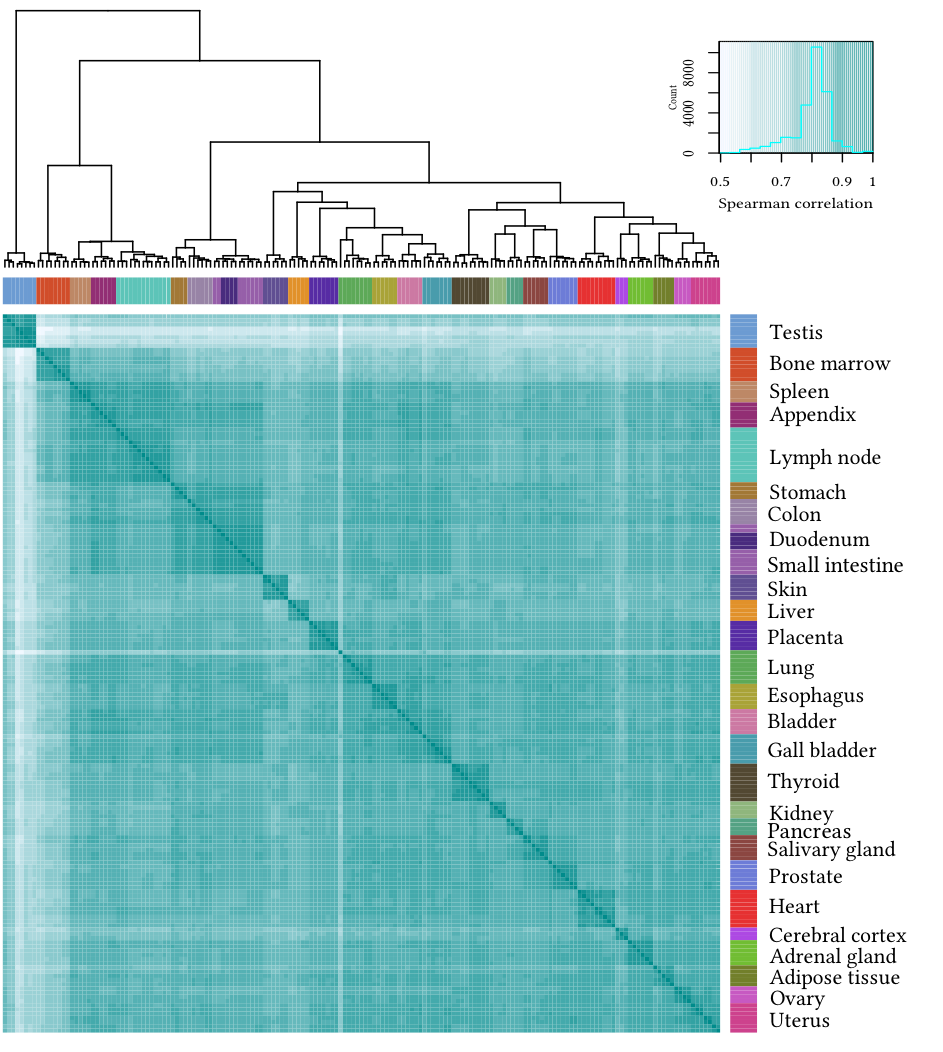
\includegraphics[width=0.9\textwidth]{expressed/FabergerAnnotated2_noLog_NoMito_htseqSpearman.png}
    \caption{Clustering based on Ward's method}\label{fig:FabergerRedone}
   \end{subfigure}

     \begin{subfigure}[hp]{0.70\textwidth}
      \centering 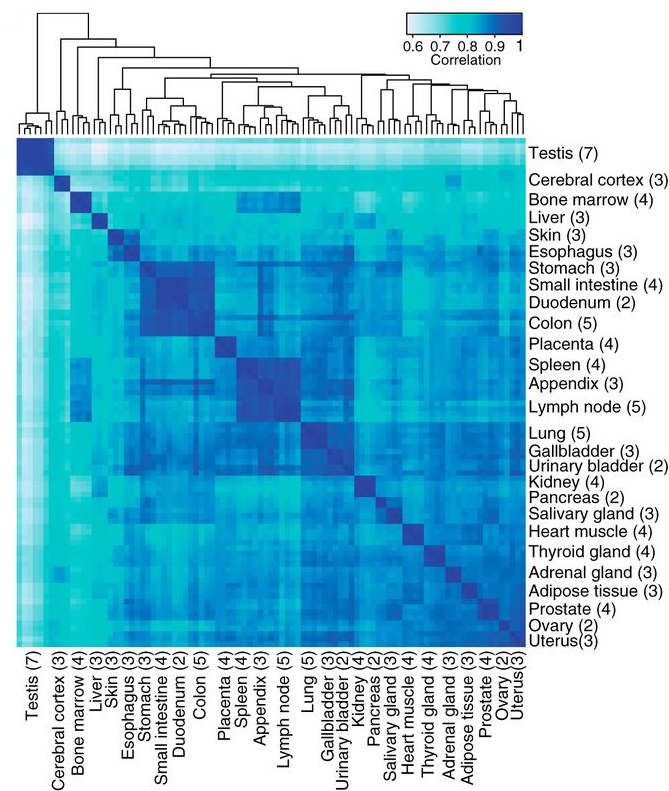
\includegraphics[width=0.9\textwidth]{expressed/FabergerOriginal.png}
      \caption{Clustering directly extracted from the original study
      {\footnotesize \mycite{Uhlen2014}}}\label{fig:fabergerOriginal}
       \end{subfigure}
    \caption[Comparison of two clustering methods on a subset of the \uhlen\ study]{%
    \textbf{Comparison of two clustering methods on a subset of the Uhlén study}.
    (\subref{fig:FabergerRedone}) includes all the samples and
    we observe that only a few of them are mixed with other samples from other tissues.
    This mixture is only observed between \tissue{Small intestine} and \tissue{Duodenum}.
 }\label{fig:versusFaberger}
\end{figure}

\section{Reducing sources of bias}\label{sec:bias_sources}

Many non-trivial methods correct for the skewness present in
\Rnaseq\ and \ms-based proteome global expression distributions
and for other possible bias sources.
For some examples, see \citet{batchEffect,Leek2014-bl,Yi2018-rv,Li2014-cv,Stegle2012-td}.

However, it may be complex to assess the biological relevance of those corrections.
Moreover, many require more metadata that is often available in the public
repositories.
In the context of this thesis, I am interested in
consistent traits across the datasets that may be consolidated into a reference.
Thus, biases that are common to all the different included studies are in practice
negligible.
On the other hand, I have adjusted for a few easily avertible biases
that I describe hereinafter.

\subsection{Mitochondria issue}\label{subsec:mito}

Gene expression levels of mitochondria can report very useful information,
\eg\ the stress level of a cell in a single cell experiment~\mycite{Ilicic2016}.
However, it is unwise to keep them for a bulk analysis, particularly when
comparing different biological sources.
Indeed, it is very hard to properly normalise their expression;
it involves knowing the amount of mitochondrial genome copies
in the studied samples, while the mitochondria are from an unknown polyploidy
and \Rnaseq\ protocols are badly suited for polyploid organisms~\mycite{Pearce2015-xa}.
Thus, I have decided to remove them from the analysis as they skew anything relying
on correlation.
In fact, there are always mitochondrial genes among the highest expressed genes
and they usually dominate manifolds the expression of the other genes.

Removing the (37) mitochondrial genes from the bulk of expressed genes
(more than 10,000 \pcgs) produces more defined clusters as showed on
\Cref{fig:MitoNomito}
(see also, in the next chapter analysis,
\Cref{fig:noMitoNoRep4T} in comparison of \Cref{fig:ExpGenePcoding1_withMito},
where the simple exclusion of the mitochondrial genes allows all tissues
to cluster by biological origin rather than the mixtures observed
when they are kept).
\Cref{fig:MitoVar} illustrates furthermore the distinctiveness
of the mitochondrial genes expression levels.

\begin{figure}[!htbp]
    \centering
    \begin{subfigure}[hp]{0.85\textwidth}
        \centering
        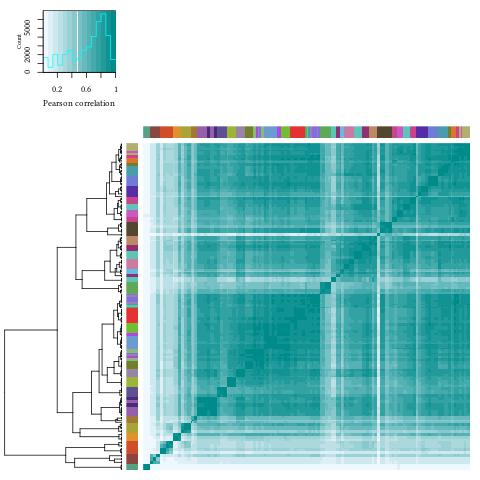
\includegraphics[width=0.85\textwidth]{expressed/Uhlen_noLog_mito_htseq.jpeg}
        \caption{With the 37 mitochondrial genes included}\label{fig:withMito}
    \end{subfigure}

    \begin{subfigure}[hp]{0.85\textwidth}
        \centering
        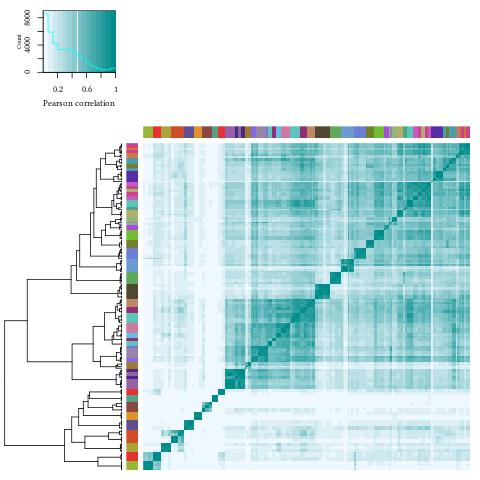
\includegraphics[width=0.85\textwidth]{%
            expressed/Uhlen_noLog_NoMito_htseqPearson.jpeg}
        \caption{Without the mitochondrial genes}\label{fig:NoMito}
    \end{subfigure}
    \caption[Clustering of the biological samples of \uhlen\
    dataset based on the Pearson correlation]{\label{fig:MitoNomito}\textbf{Clustering
    of the biological samples of Uhlén study based on the Pearson correlation}
    --- all expressed genes are included.}
\end{figure}

\subsection{Protein-coding genes only}\label{subsec:protcodingOnly}
\vspace{-0.3in}
I have focused my analyses on the \mRNAs\ (\ie\ \glspl{RNA} that have a
biotype described as \emph{\pc} in \ens{76}).

In addition to the obvious reason to match with the proteomic data,
most of the transcriptomic data is the product of poly-A selected protocols
(see \Cref{msec:polyA}: \nameref{msec:polyA}).
Thus, aside from the \mRNAs, all the other \glspl{RNA} are off-target
and, for many of them,
their expression levels estimations may be highly imprecise.

\vspace{-0.1in}
\subsection{Expressed or not expressed}\label{sec:ExpressedOrNot}
\vspace{-0.3in}
\begin{figure}[!htb]
    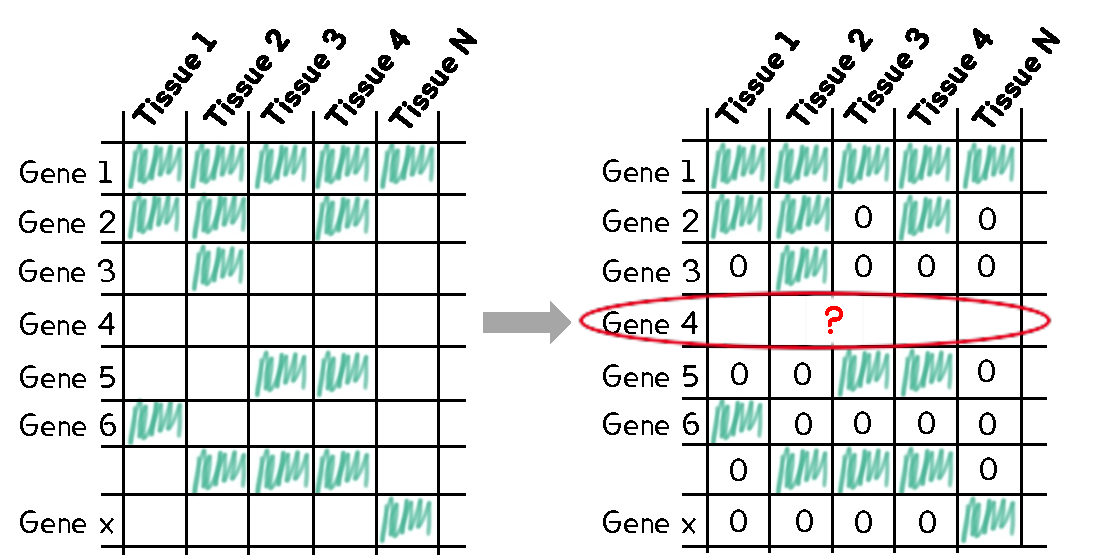
\includegraphics[scale=0.7]{expressed/expressedNotExp.pdf}\centering
      \caption[Expressed or not: several cases illustrated]
      {\label{fig:DefineExpression}\textbf{Expressed or not: several cases
      illustrated.}\smallbreak{} Genes like \emph{Gene 1} are unequivocal: they have been
      detected in all the different tissues. Genes that have been quantified in
      \emph{some} of the conditions are, in principle, detectable with the
      protocol of sampling and quantification used for the assay.
      For these genes, when no signal is collected, I assume this is a true $0$ signal.
      In contrast, genes without any quantification
      in any tissue, \eg\ \emph{Gene 4}, are discarded from the remaining analysis as
      it is impossible to state
      whether they are truly absent from the biological sample or if it is due
      to the protocol used; they are \emph{undefined}. The same approach is used
      for the transcriptome and the proteome.}
\end{figure}

While it can seem a trivial concept and might be overlooked, whether a specific
molecule is truly expressed --- or not --- in a given condition, can actually have
an extensive impact on the results of the analyses, particularly when integrating
proteome and transcriptome together.

For example, the Pearson correlation coefficient is very
sensitive to outliers and null values. If for both samples, a vast number of
null values are recorded, this will lead to a greater similarity.
Hence, it is important that the data used for the analysis is meaningful in
its entirety, \ie\ a null value is a truly an observation and translates to
a lack of expression, rather than a lack of observation.

\begin{itemize}
        \item\textbf{The undefined}:\label{subsec:ExpressedOrNot-undefined} %\KOMAoptions{parskip=false}
        If a protein or transcript is never found in any of the samples of a dataset,
        then I considered that we can not determine if the protein or transcript was
        either truly not expressed or, for any reason, was not captured during the library
        preparation or the identification/quantification steps. Hence, those are
        excluded from the analyses as I can not resolve precisely if this is a
        technical artefact or a biological truth. An example is illustrated by the row
        circled in red in~\Cref{fig:DefineExpression}.
        \item\textbf{Expression in a dataset}:\label{subsec:ExpressedOrNot--expDataset} %
        By contrast, if a protein or a transcript is expressed in some samples of the
        dataset, then, whenever no expression was recorded in the other
        samples, I consider that the expression of the considered macromolecule is truly
        null for those samples.
        \item\textbf{Expression within a sample}:
        Due to the technical (and biological) differences between proteomics and
        transcriptomics, I use different thresholds to classify the presence of
        a protein or a transcript.
        \begin{itemize}
                \item\textsf{Expressed protein}:
                On the proteomic side, I consider that a protein is expressed
                if it has been identified and quantified.
                In other words, a protein is expressed
                if the expression value is greater than zero in a sample.
                \item\textsf{Expressed transcript}:\label{subsubsec:exprTrans} %
                It is a bit more complex on the transcriptomic side as
                we have to account for technical noise,
                but also \enquote{transcriptional noise}~\mycite{rnaseq-2009,lowNoiseLimit}.
                Indeed, \citet{seqcmaqc} reports that
                excluding low-expression measurements reduce the \gls{FDR}
                of \glspl{RNA} considerably.\\
                While we can empirically evaluate it for each \Rnaseq\
                dataset~\mycite{ramskoldan:2009},
                there is a widespread threshold used in the literature:
                1 \gls{FPKM} (or \gls{RPKM}) --- \eg{}~\citet{Uhlen2014,Uhlen2015}.
                In fact, \citet{Hebenstreit:2011} showed in their study
                \paper{\citetitle{Hebenstreit:2011}},
                that to be detected and quantified at protein level,
                a \mRNA\ should at least present an expression equals to 1 \gls{RPKM}.\\
                As an important part of my thesis focuses on
                the comparison of proteomic and transcriptomic data (see \Cref{ch:Integration}),
                I have conducted all the analyses at least once with this threshold of $1$ \gls{FPKM}
                (I have also used $0$ (\ie\ using the same threshold for \mRNAs\
                for the proteins) and $5$ \FPKM\ as other thresholds
                for a few specific analyses).
        \end{itemize}
\end{itemize}

\minisec{Limitation of the study}
\vspace{-0.1in}
Although I have compared the list of
undefined, expressed and unexpressed molecules,
the bulk of the analyses has been done on the common expressed genes across
the datasets.

In other words, a \mRNA\ --- or protein --- was excluded
if it is not expressed in at least
one sample in \emph{each and every} dataset used for the analyses,
I then exclude it.
This led me to define different working sets for the following chapters analyses
to limit the number of omitted \mRNAs/proteins.

\subsection{Aggregating tissue expression}\label{subsec:averagedTissue}
\vspace{-0.15in}
To avoid unnecessary skewness in the meta-analyses due to
imbalanced number of
biological replicates across the datasets (see \Cref{sec:expDesign}:
\nameref{sec:expDesign}),
I computed a \emph{\enquote{virtual} reference} for each tissue
within the datasets that present more than one biological sample per tissue,
\ie\ \vt, \uhlen\ and \gtex\ datasets.
Note that, \castle, \cutler, \kuster\ and \pandey\ datasets present by design only
one measure of expression per gene per tissue.

To compute the \enquote{virtual} references for \vt, \uhlen\ and \gtex\ datasets,
I have taken the median value of each gene across all the
biological replicates for each of their tissues.



\textbf{Notes:}
\KOMAoptions{parskip=never}
\begin{itemize}[topsep=0pt,nosep]
        \item For \ibm\ dataset, I have discarded the single-end sequenced samples
            (as already mentioned in \Cref{ch:datasets}).
        \item The \uhlen\ dataset required an extra \latin{a priori} step to
            the averaging of the biological replicates
            for some of the tissues as they present technical replicates.
            For these, I have first averaged the gene expression levels
            for each subject-tissue pair before computing
            the gene expression level medians of each tissue.
        \item The \gtex\ dataset required another \emph{post}-processing
            step after the averaging of the biological replicates.
            Indeed, the samples are described based on their
            body site sources while the other datasets describe their samples
            only based on their tissue origin.
            Thus, while there is only \tissue{Heart} samples in \castle, \vt,
            \ibm, \uhlen, \cutler, \kuster\ and \pandey,
            \gtex\ has samples from the \tissue{left ventricle of the Heart}
            and from the \tissue{Atrial appendage of the Heart}.
            For this case and other similar ones,
            I have average the virtual reference of the body sites in \gtex\
            that I considered relevant for comparison with tissues found
            in the other datasets.
        \item While I have detected many samples that seem outliers to their
            biological replicates within the same datasets,
            I have decided to keep all the samples for the tissues expression
            averaging step. On this matter,
            in many scientific exchanges,
            I was repetitively asked about the inclusion of all the \gtex\ dataset samples
            related to \tissue{Oesophagus} for the averaging step.
            Indeed, while two of the three \gtex{}'s body sites
            (\ie\ \tissue{Gastro oesophageal junction} and \tissue{Oesophageal muscularis})
            present great similarities together ($r = 0.99$) and more modest correlations
            to \uhlen{}'s \tissue{Oesophagus} samples ($r < 0.80$),
            the last body site (\ie\ \tissue{Oesophageal muscularis}) expression,
            very dissimilar to the two former ones ($r < 0.64$),
            presents higher correlation to \uhlen's ($r = 0.94$).
            Thus, while only considering this latter body site significantly improves
            the overall \oesophagus\ correlation between \gtex\ and \uhlen,
            I have decided to include all three body sites (as one tissue)
            in my study.
            Indeed, there are no suitable reasons or information that allows excluding
            any of the body site \latin{prior} to the analyses;
            gene expression scatter plots of the \uhlen{}'s samples versus
            any of these three body sites present two trends which suggest that
            \uhlen{}'s \oesophagus\ samples are composite.

%see more for esophagus in next chapter.
\end{itemize}
\KOMAoptions{parskip=half*}

\label{def:trep}
The meta-analyses of the following chapters use
a \glsxtrfull{TREP} for each tissue of each study, \ie\
there is only one measure per gene for each tissue.
These measures are either
the primary sample expressions for \castle\ and \ibm\ studies or
these \emph{\enquote{virtual}} constructed \emph{references}
for \brawand, \uhlen\ and \gtex.



\section{Discussion and Conclusion}

In this chapter, I have reviewed many fine quality control points that
may be (and often are) overlooked.
While it may be perceived as nitpicking,
these details have critical impact on the results of the analyses
I perform and more gravely on their interpretations\footnote{%
For more, see~\paper{\citetitle{Kratz2014}}~\mycite{Kratz2014}
and the included references.}.

Aside the datasets selection criteria,
this phase is by far the most subjective one of the whole thesis.
Hence, to avoid excessive \emph{data cleaning}
and possible cognitive biases,
I have formulated the aforementioned filtering rules
that are important but simple.

Overall, I am quite stringent and I have preferred to keep more data
without any strong rationale to discard them.
Therefore, there are sharper filters and samples exclusion options that
may easily improve the results I present in this thesis.


\begin{comment}
\section{Methods}

All the analysis have been run in R version 3.4.2 (2017-09-28)
Platform: x86_64-apple-darwin15.6.0 (64-bit)
Running under: OS X El Capitan 10.11.6
and \TK{EBI cluster}.

R version 3.4.2 (2017-09-28)
Platform: x86_64-apple-darwin15.6.0 (64-bit)
Running under: OS X El Capitan 10.11.6

Matrix products: default
BLAS: /System/Library/Frameworks/Accelerate.framework/Versions/A/Frameworks/vecLib.framework/Versions/A/libBLAS.dylib
LAPACK: /Library/Frameworks/R.framework/Versions/3.4/Resources/lib/libRlapack.dylib

locale:
[1] en_GB.UTF-8/en_GB.UTF-8/en_GB.UTF-8/C/en_GB.UTF-8/en_GB.UTF-8

attached base packages:
 [1] stats4    parallel  grid      stats     graphics  grDevices utils     datasets  methods   base

other attached packages:
 [1] topGO_2.28.0          SparseM_1.77          GO.db_3.4.1           org.Hs.eg.db_3.4.1    AnnotationDbi_1.38.2
 [6] IRanges_2.10.5        S4Vectors_0.14.7      Biobase_2.36.2        clusterProfiler_3.4.4 DOSE_3.2.0
[11] Rgraphviz_2.20.0      graph_1.54.0          BiocGenerics_0.22.1   VennDiagram_1.6.17    futile.logger_1.4.3
[16] gridExtra_2.3         mgcv_1.8-22           nlme_3.1-131          scales_0.5.0          WGCNA_1.61
[21] fastcluster_1.1.24    dynamicTreeCut_1.63-1 gplots_3.0.1          reshape2_1.4.2        extrafont_0.17
[26] ggplot2_2.2.1

loaded via a namespace (and not attached):
 [1] bitops_1.0-6          matrixStats_0.52.2    robust_0.4-18         fit.models_0.5-14     bit64_0.9-7
 [6] doParallel_1.0.11     RColorBrewer_1.1-2    tools_3.4.2           backports_1.1.1       DT_0.2
[11] rpart_4.1-11          KernSmooth_2.23-15    Hmisc_4.0-3           DBI_0.7               lazyeval_0.2.0
[16] colorspace_1.3-2      nnet_7.3-12           bit_1.1-12            compiler_3.4.2        preprocessCore_1.38.1
[21] extrafontdb_1.0       htmlTable_1.9         labeling_0.3          caTools_1.17.1        checkmate_1.8.4
[26] DEoptimR_1.0-8        mvtnorm_1.0-6         robustbase_0.92-7     stringr_1.2.0         digest_0.6.12
[31] foreign_0.8-69        rrcov_1.4-3           base64enc_0.1-3       pkgconfig_2.0.1       htmltools_0.3.6
[36] htmlwidgets_0.9       rlang_0.1.2           RSQLite_2.0           impute_1.50.1         jsonlite_1.5
[41] BiocParallel_1.10.1   gtools_3.5.0          GOSemSim_2.2.0        acepack_1.4.1         magrittr_1.5
[46] Formula_1.2-2         Matrix_1.2-11         Rcpp_0.12.13          munsell_0.4.3         stringi_1.1.5
[51] yaml_2.1.14           MASS_7.3-47           qvalue_2.8.0          plyr_1.8.4            blob_1.1.0
[56] DO.db_2.9             gdata_2.18.0          lattice_0.20-35       splines_3.4.2         knitr_1.17
[61] igraph_1.1.2          fgsea_1.2.1           codetools_0.2-15      fastmatch_1.1-0       futile.options_1.0.0
[66] glue_1.1.1            latticeExtra_0.6-28   lambda.r_1.2          data.table_1.10.4-1   foreach_1.4.3
[71] Rttf2pt1_1.3.4        purrr_0.2.3           tidyr_0.7.1           gtable_0.2.0          survival_2.41-3
[76] pcaPP_1.9-72          tibble_1.3.4          rvcheck_0.0.9         iterators_1.0.8       memoise_1.1.0
[81] cluster_2.0.6

\end{comment}
